\documentclass{article}
\usepackage[english]{babel}
\usepackage{amsmath,amssymb,amsthm,upref}
\usepackage{tikz}
\usepackage{graphicx}
\usepackage{listings, color}
\lstdefinestyle{Java}{
  belowcaptionskip=1\baselineskip,
  breaklines=true,
  frame=L,
  xleftmargin=\parindent,
  language=C,
  showstringspaces=false,
  basicstyle=\footnotesize\ttfamily,
  keywordstyle=\bfseries\color{green!40!black},
  commentstyle=\itshape\color{purple!40!black},
  identifierstyle=\color{blue},
  stringstyle=\color{orange},
}
\title{Title}
\author{your name\thanks{for instance : ak223wd}}
\date{dd/mm/yyyy}
\begin{document}
%1)
\maketitle
\tableofcontents
\section{name of the section}
\subsection{name of the subsection}
\subsubsection{subsubsection1}
\section{Section 2}
\subsection{subsection 2}
\subsubsection{subsubsection1}

\textup{Upright text}

\textit{italic text}

\textsl{slanted text}

\textbf{bold text}

\textsf{Sanserif text}

\textsc{Small caps text}

\texttt{type write text}

\begin{abstract}
A short text describing the contents of the document. 
\end{abstract}

%1.1)List
\begin{enumerate}
\item first part list 
\item second part
\item third part
\end{enumerate}

\begin{itemize}
\item Section 1 list
\begin {itemize}
\item Subsection 1 list 
\item Subsection 2
\end{itemize}
\item Section 2
\end {itemize} 

%2)
\begin{equation*}
\frac {\sin mx}{\sin x} = (-4)^{{(m-1)}/{2}}\prod_{j=1}^{{(m-1)}/{2}}(\sin^{2}x - \sin^{2}\frac{2\pi \, j}{m})
\end{equation*}
$f_{n} = f_{n-1} + f_{n-2}$ 


\break

%3)
\begin{tabular}{l l l r@{.}l}
\hline 
& & \multicolumn{3}{c}{\textbf{World Record}} \\ 
\cline{3-5}
\bfseries{Name} & \bfseries{Country} & \bfseries{Event} & \multicolumn{2}{c}{\bfseries{Result}}				 \\ 
\hline Anna-Karin Kammerling & Sweden & 50 m butterfly & 25&57 \\ 
Wilson Kipketer & Denmark & 800 m & 2:11&96 \\ 
Jan 
\v{Z}elezný & Czech Republic & javelin throw & 98&5 \\ 
Sergei Bubka & Ukraine & pole vault & 6&14 \\ 
\hline 
\end{tabular}  

%4)
\begin{table}[htbp]
\centering
\begin{tabular}{l l l r@{.}l}
\hline 
& & \multicolumn{3}{c}{\textbf{World Record}} \\ 
\cline{3-5}
\bfseries{Name} & \bfseries{Country} & \bfseries{Event} & \multicolumn{2}{c}{\bfseries{Result}}				 \\ 
\hline Anna-Karin Kammerling & Sweden & 50 m butterfly & 25&57 \\ 
Wilson Kipketer & Denmark & 800 m & 2:11&96 \\ 
Jan 
\v{Z}elezný & Czech Republic & javelin throw & 98&5 \\ 
Sergei Bubka & Ukraine & pole vault & 6&14 \\ 
\hline 
\end{tabular}  
\caption{World Record and Results} 
\label{Table 1} 
\end{table} 

As the table \ref{Table 1} shows.

\break

%5)
\begin{center}
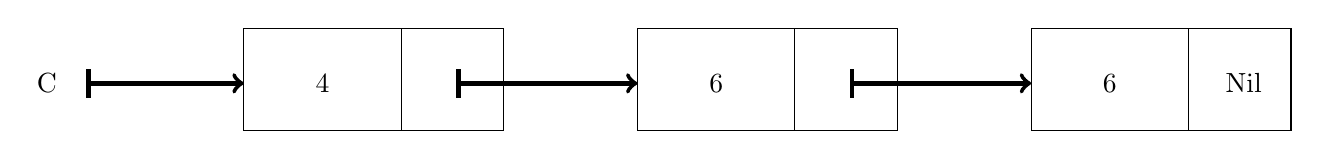
\begin{tikzpicture}
\draw (-0.5,0.6) node{C};
\draw [| ->, ultra thick] (0,0.6) -- (2,0.6);

\draw (2,0) rectangle (4,1.3);
\draw (3,0.6) node{4};
\draw (4,0) rectangle (5.3,1.3);
\draw [| ->, ultra thick] (4.7,0.6) -- (7,0.6);

\draw (7,0) rectangle (9,1.3);
\draw (8,0.6) node{6};
\draw (9,0) rectangle (10.3,1.3);
\draw [| ->, ultra thick] (9.7,0.6) -- (12,0.6);

\draw (12,0) rectangle (14,1.3);
\draw (13,0.6) node{6};
\draw (14,0) rectangle (15.3,1.3);
\draw (14.7,0.6) node{Nil};

\end{tikzpicture}
\end{center}

The figure \ref{tikzT} about TikZ Typeset is also available
%7)Floating Environment TipZ
\begin{figure}
\begin{center}
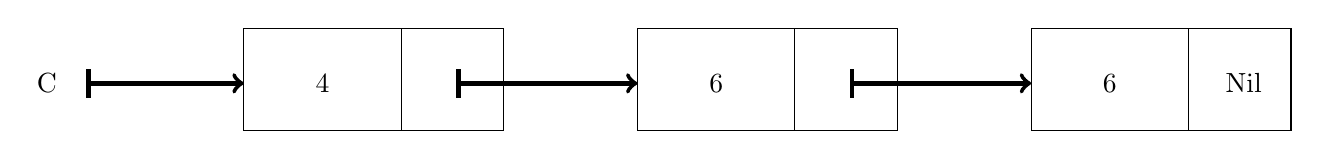
\begin{tikzpicture}
\draw (-0.5,0.6) node{C};
\draw [| ->, ultra thick] (0,0.6) -- (2,0.6);

\draw (2,0) rectangle (4,1.3);
\draw (3,0.6) node{4};
\draw (4,0) rectangle (5.3,1.3);
\draw [| ->, ultra thick] (4.7,0.6) -- (7,0.6);

\draw (7,0) rectangle (9,1.3);
\draw (8,0.6) node{6};
\draw (9,0) rectangle (10.3,1.3);
\draw [| ->, ultra thick] (9.7,0.6) -- (12,0.6);

\draw (12,0) rectangle (14,1.3);
\draw (13,0.6) node{6};
\draw (14,0) rectangle (15.3,1.3);
\draw (14.7,0.6) node{Nil};

\end{tikzpicture}
\end{center}
\caption{TikZ Typeset Example}
\label{tikzT}
\end{figure}


\break
%6)
\begin{center}
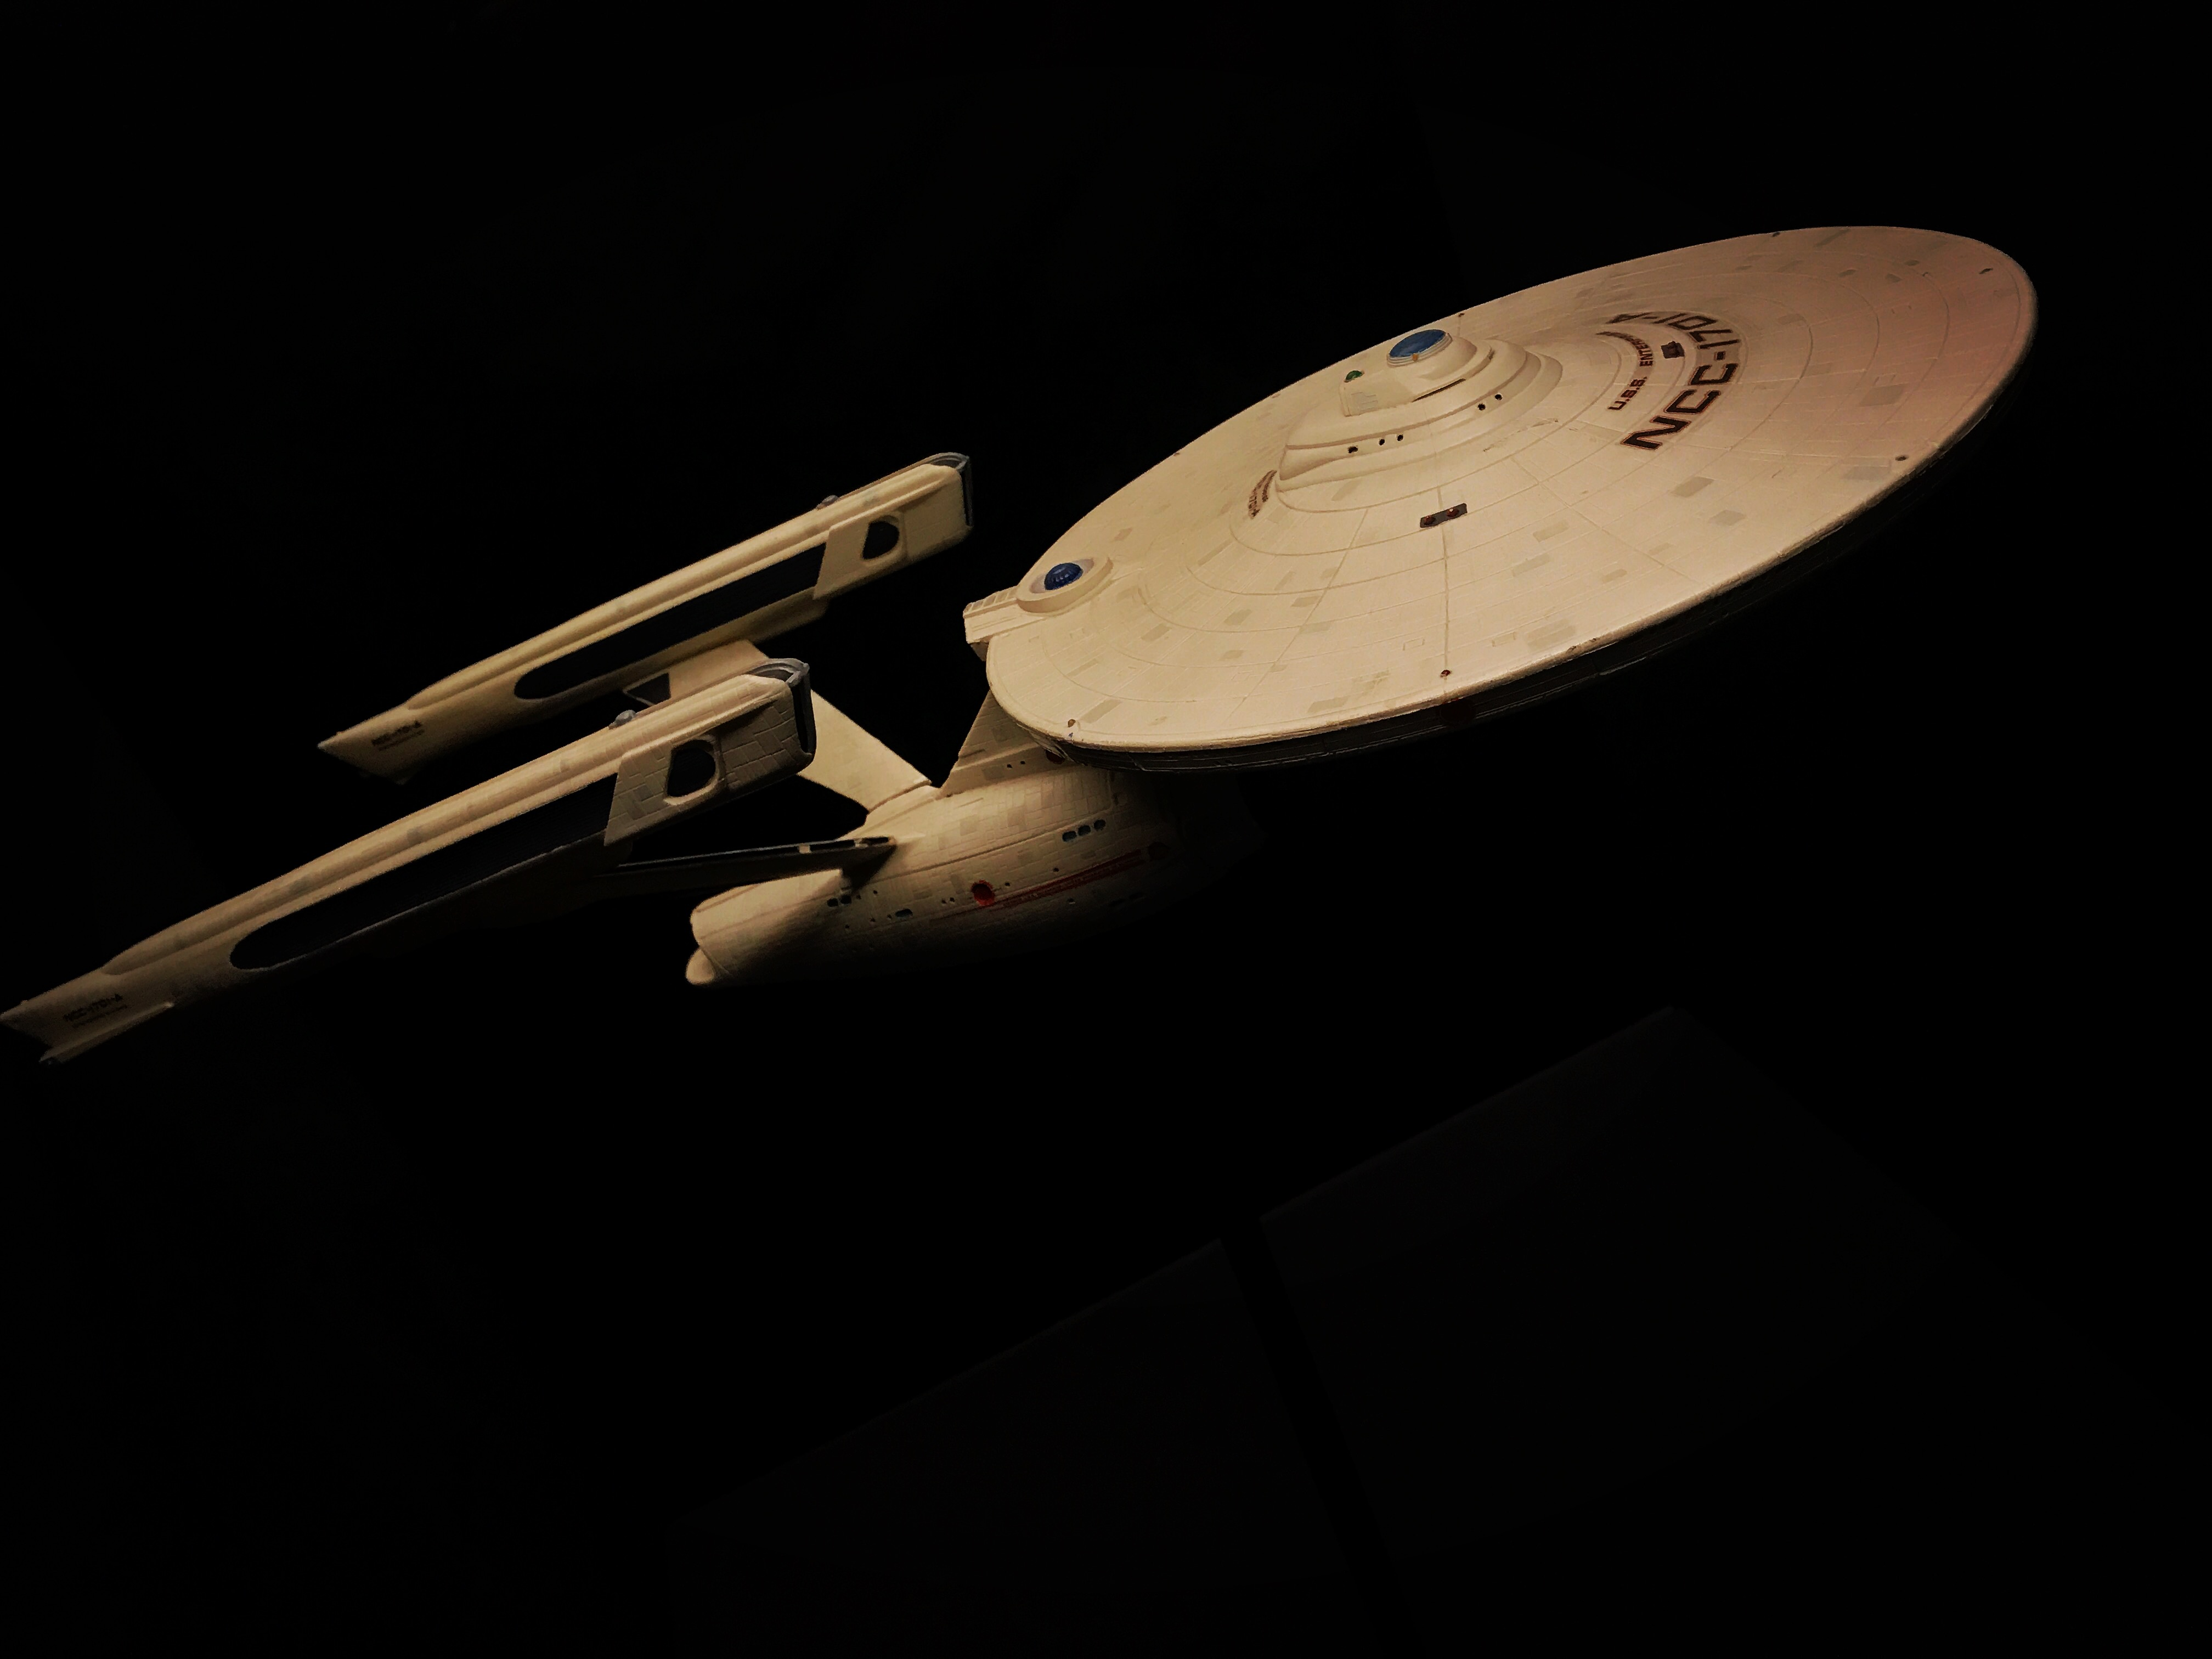
\includegraphics[width = 5cm, height=5cm]{IMG_7052.JPG}
\end{center}
%7)Floating Environnement Image 
\begin{figure}
\begin{center}
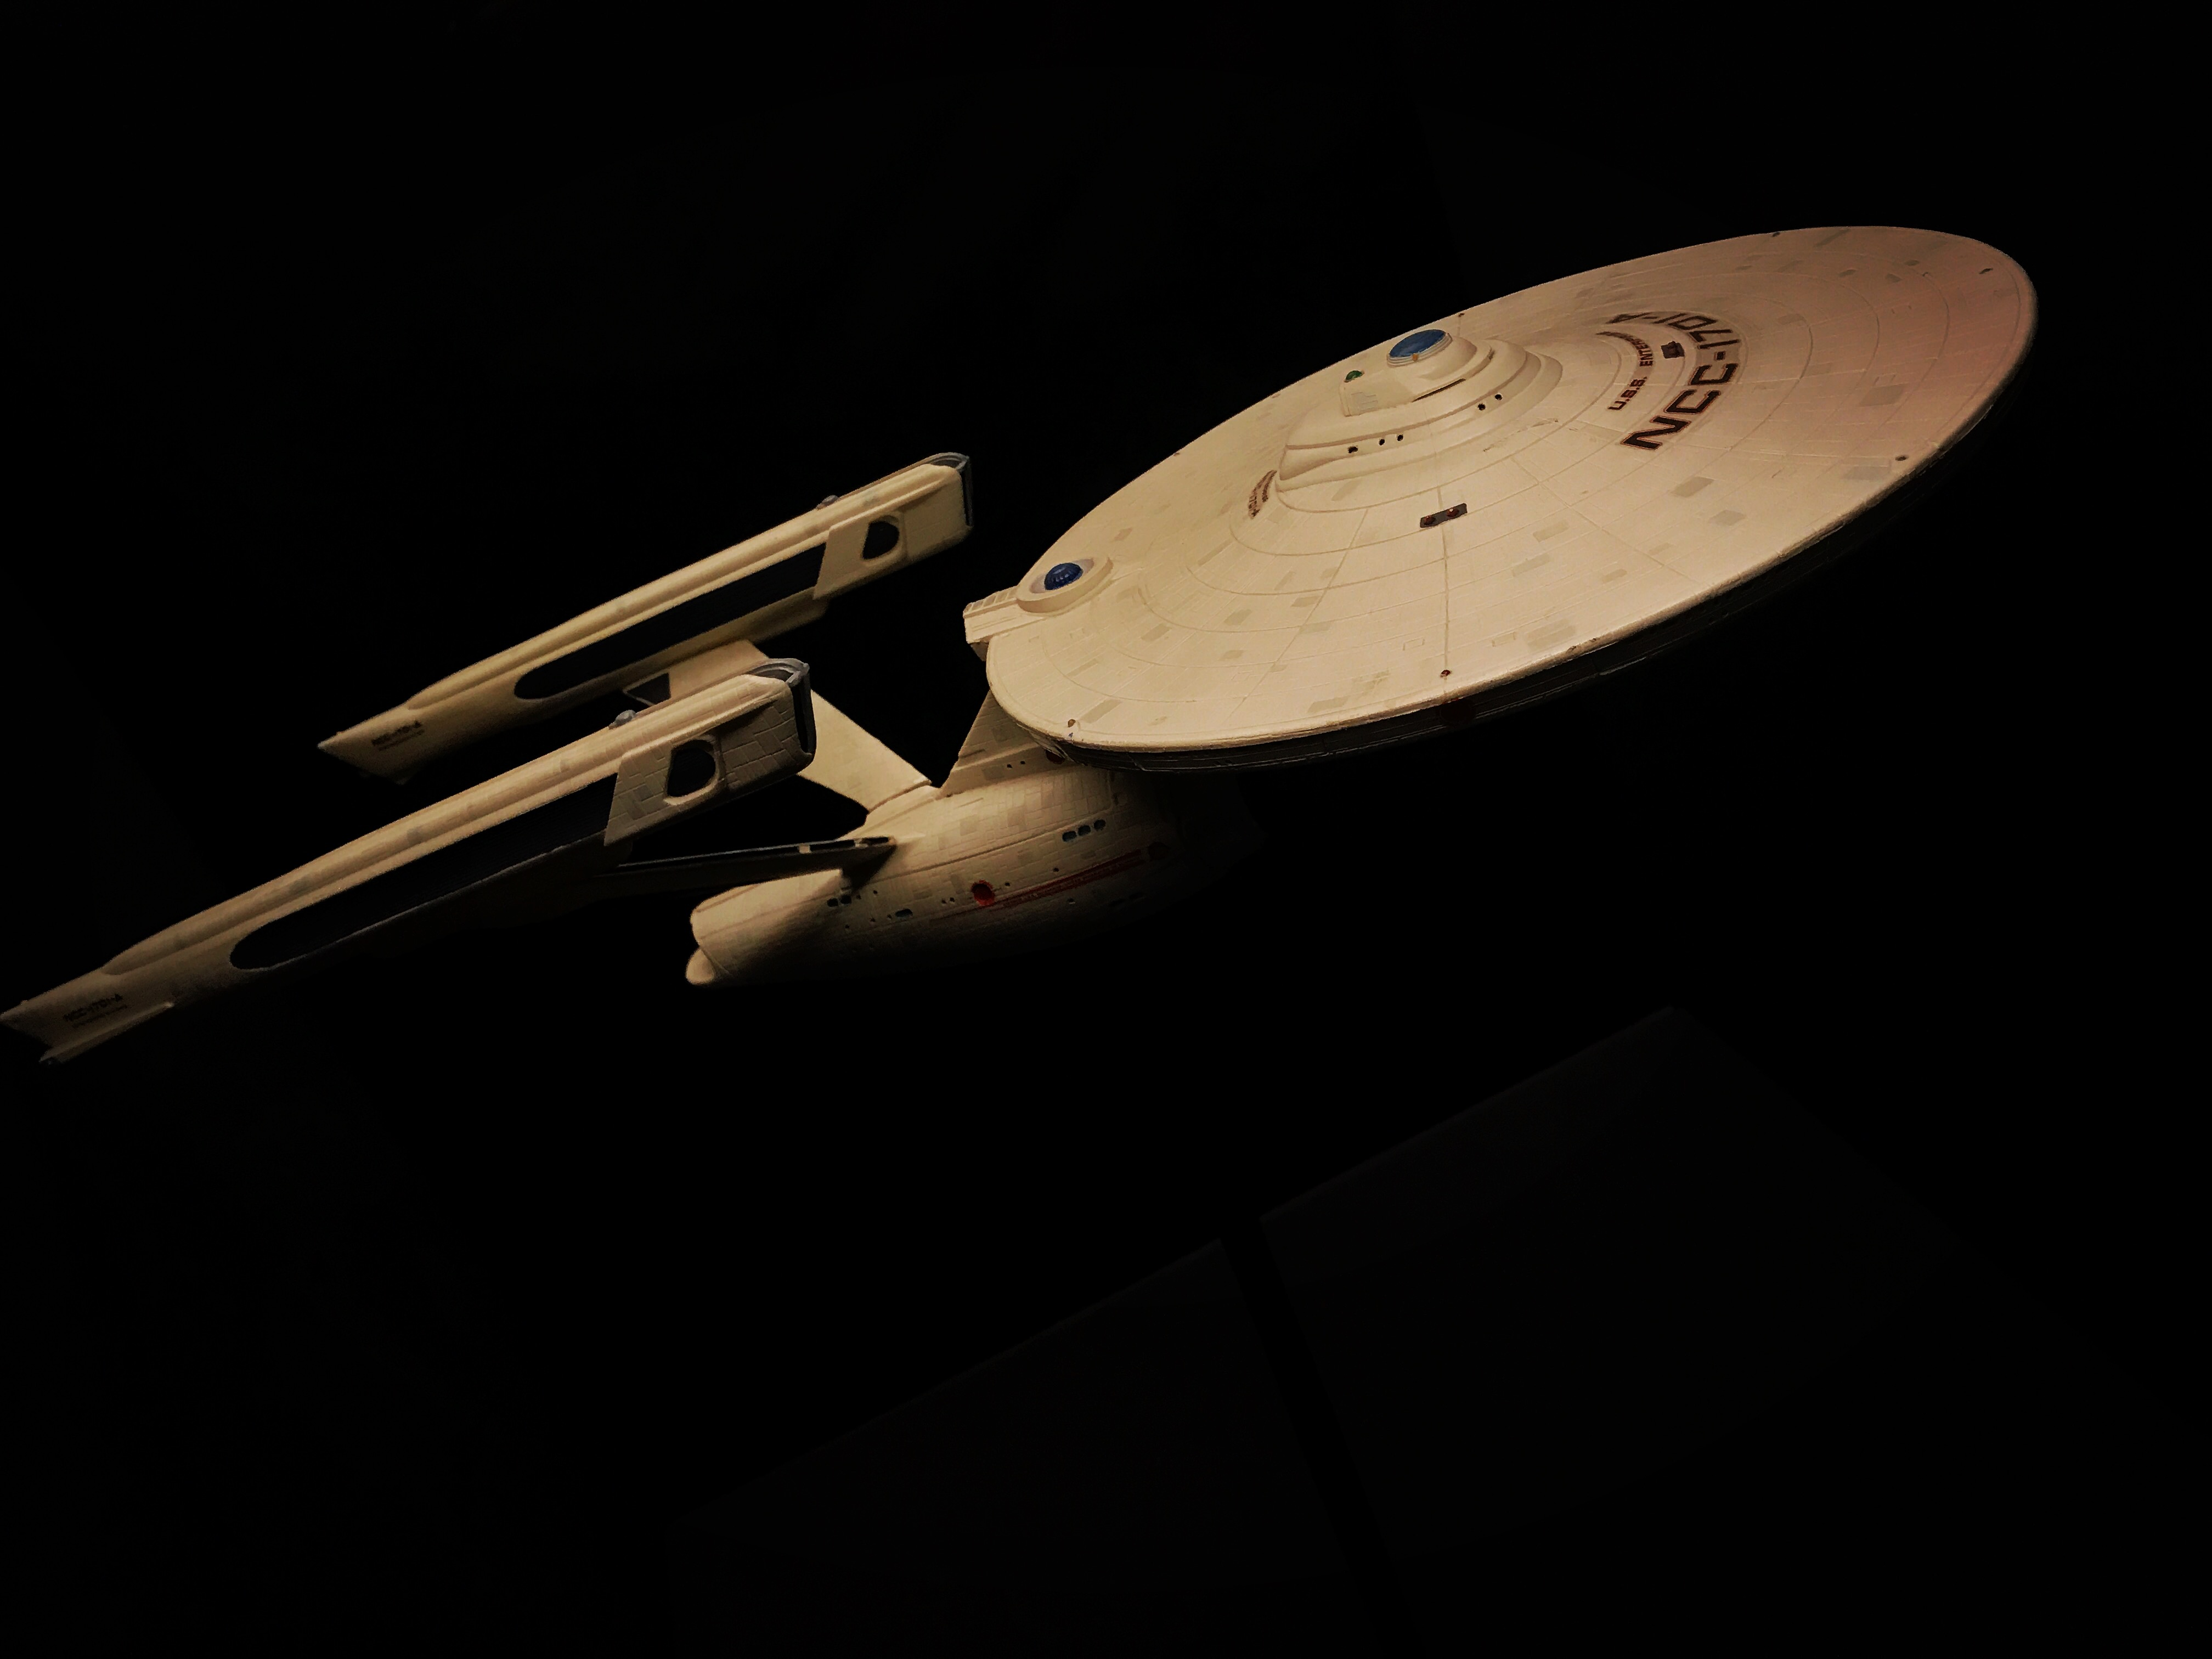
\includegraphics[width = 5cm, height=5cm]{IMG_7052.JPG}
\end{center}
\caption{Star Trek Spacecraft taken by ak223wd (me) in Science Museum of London}
\label{Star Trek Spacecraft}
\end{figure}
The  figure (image) \ref{Star Trek Spacecraft} represents a spacecraft from Star Trek.

\break

%9)
\lstset{style=Java}

\begin{lstlisting}
import java.util.Scanner;

public class CountA {

    public static void main(String[] args) {
        Scanner sc = new Scanner(System.in);
        //Ask for a line of text
        System.out.print("Provide a line of text : ");
        String text = sc.nextLine();
        sc.close();
        //System.out.print(text);


        //How many 'a' and 'A' the text contains
        char letter = 'a';
        char letA = 'A';

        int count = 0;
        int count2 = 0;

        for (int i=0;i<text.length();i++) {

            if(text.charAt(i) == letter) {
                count++;
            }
            else if (text.charAt(i)==letA) {
                count2++;
            }


        }
        System.out.println("Number of \'a\' : " +count);
        System.out.println("Number of \'A\' : " +count2);

    }
}
\end{lstlisting}
%10)
\newcommand{\summation}[2]{\sum_{i=0}^{#1}{#2}_i}

\begin{equation}
\summation{n}{\alpha}
\summation{10}{\gamma}
\summation{50}{\beta}
\end{equation}

%11)
Peter J.Cameron\cite{Peter J.Cameron}
Patrick Morton\cite{Patrick Morton}

\begin{thebibliography}{2}
\bibitem[1]{Peter J.Cameron}P.J.Cameron, \emph{Permutations Groups}. Cambridge : Cambridge University Press, 1999.

\bibitem[2]{Patrick Morton} P. Morton, "Periods of Maps or Irreducible Polynomials over Finite Field", \emph{Finite Fields and their Applications (Finite Fields Appl.)}, vol. 3, pp. 11-24, 1997.
\end{thebibliography}

\break
%8) Correction
%a)
$x^{n^{2}} + y^{n+1} = z^{n}$
%b)
\begin{center}
\emph{The Johansson Brothers \& Son}
\end{center}
%c)
..end of paragraph 

	A new paragraph...



%\newpage
%7)

\end{document}